
% This LaTeX was auto-generated from MATLAB code.
% To make changes, update the MATLAB code and republish this document.

\documentclass[11pt]{article}
\usepackage[utf8]{inputenc}
\usepackage[T1]{fontenc}
\usepackage{amsthm}
\usepackage{enumitem}
\usepackage{amssymb}
\usepackage{amsmath}
\usepackage{amsfonts}
\usepackage[version=4]{mhchem}
\usepackage{stmaryrd}
\usepackage{mathrsfs}
\usepackage{bm}
\usepackage{graphicx}
\usepackage[export]{adjustbox}
\graphicspath{ {./images/} }
\usepackage{algorithm}
\usepackage{algorithmic}
\usepackage{makecell}  % 表格换行
\usepackage{tikz}


\usepackage{hyperref}
\hypersetup{
    colorlinks=true,     % 启用颜色链接
    linkcolor=blue,     % 内部链接的颜色
    citecolor=blue,      % 引用文献的颜色
    urlcolor=blue,       % URL链接的颜色
    linktoc=red,      % 不影响目录链接颜色
}

\usepackage[a4paper, top=1in, bottom=1in, left=1in, right=1in]{geometry}

\title{
{\bf \huge Notes on M\"untz-Jackson Theorem}
%{\bf \large For M\"untz systems on [0,1]}
}
\author{Huaijin Wang}
\date{December 10, 2024}


\begin{document}


\newtheorem{definition}{Definition}[section]
\newtheorem{property}{Property}[section]
\newtheorem{lemma}{Lemma}[section]
\newtheorem{theorem}{Theorem}[section]
\newtheorem{corollary}{Corollary}[section]
\newtheorem{remark}{Remark}[section]
\newtheorem{example}{Example}[]
\newtheorem{notation}{Notation Declaration}[]
\newtheorem{question}{Question}[]
\newtheorem{exercise}{Exercise}[section]
\newtheorem{exercise*}{Exercise}[]

%\maketitle




\newpage



\begin{exercise*}
Consider the BVP
\begin{equation}
\left \{
\begin{aligned}
& -u^{\prime \prime} = f,\quad x\in \Lambda := (0,1), \\
& u(0)=0,\ u^{\prime} (1) = \beta.
\end{aligned}
\right .
\label{eq:1}
\end{equation}
Construct a $P1-$FEM for this problem and compare with central finite difference scheme.
\end{exercise*}
\begin{proof}[Solution]
~\\
\noindent $1.$ $P1-$FEM. 
\begin{enumerate}[label=1.\arabic*]
\item Variational form. Let $V = \{v\in H^1(\Lambda): v(0)=0\}$. Then the variational form reads
\begin{equation}
\left \{
\begin{aligned}
& \text{find}\ u\in V \ \text{s.t.}\\
& a(u,v) = \mathcal{F}(v),\ \forall v\in V,
\end{aligned}
\right .
\label{eq:vp}
\end{equation}
where $a(u,v) = (u^\prime, v^\prime)$ and $\mathcal{F}(v) = (f,v) + \beta v(1)$. Clearly, the weak problem \eqref{eq:vp} is equivalent to the strong problem \eqref{eq:1}. The well-poseness of \eqref{eq:vp} is guaranteed by Lax-Milgram theorem.

\item Galerkin approximation. Let $V_h \subset V$ be a finite dimensional space. Replacing $V$ with $V_h$ in \eqref{eq:vp} leads to the Galerkin approximation
\begin{equation}
\left \{
\begin{aligned}
& \text{find}\ u_h\in V_h \ \text{s.t.}\\
& a(u_h, v_h) = \mathcal{F}(v_h),\ \forall v_h\in V_h.
\end{aligned}
\right .
\label{eq:ga}
\end{equation}

\item $P1$ finite element space. Let $\{x_i\}_{i=0}^N$ be the uniform grid on $\Lambda$ shown as follows:

\begin{center}
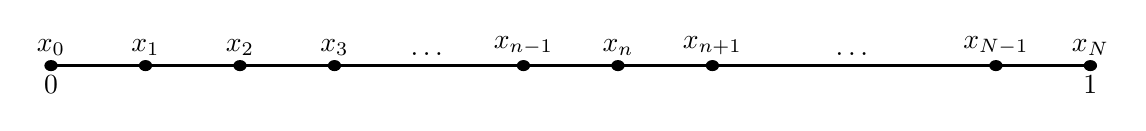
\begin{tikzpicture}[xscale=1.2, yscale=1, thick]
\draw[-] (0,0) -- (11,0);
 \foreach \x in {0,...,3} {
 \fill (\x,0) circle (2pt); % 圆点
 \node[above] at (\x,0) {$x_{\x}$};
 }
 \node[above] at (4,0) {$\dots$};
 \fill (5,0) circle (2pt);
 \node[above] at (5,0) {$x_{n-1}$};
 \fill (6,0) circle (2pt);
 \node[above] at (6,0) {$x_{n}$};
 \fill (7,0) circle (2pt);
 \node[above] at (7,0) {$x_{n+1}$};
 
 \node[above] at (8.5,0) {$\dots$};

 \fill (10,0) circle (2pt);
 \node[above] at (10,0) {$x_{N-1}$};
 \fill (11,0) circle (2pt);
 \node[above] at (11,0) {$x_{N}$};
 
 \node[below] at (0,0) {$0$};
 \node[below] at (11,0) {$1$};
\end{tikzpicture}
\end{center}

Let $\mathcal{T}_h = \{I_i \}_{i=1}^N$, where $I_i=(x_{i-1},x_i)$ is the element with length of $h=h_i:=x_i-x_{i-1}$ for $i=1,\cdots,N$. Then the $P1$ finite element space is 
\[
X_h^1 = \left \{ v\in C^0(\bar{\Lambda}): v|_{K} \in \mathbb{P}_1,\ \forall K\in \mathcal{T}_h \right \},
\]
where $\mathbb{P}_1$ is the space of polynomials degree of at most $1$. We construct a nodal basis for $X_h^1$, defined by nodes within each element. The number of nodes per element depends on the degrees of freedom, which are determined by the required polynomial degree.
\begin{equation}
\varphi_0 (x) = \left \{
\begin{aligned}
&\frac{x_1-x}{x_1-x_0}, &\quad x\in I_1,\\
& 0, &\quad \text{else},
\end{aligned}
\right.
\qquad 
\varphi_{N}(x) = \left\{
\begin{aligned}
& \frac{x-x_{N-1}}{x_{N}-x_{N-1}}, & \quad x\in I_{N}, \\
& 0,& \text{else} ,
\end{aligned}
\right .
\label{eq:basis1}
\end{equation}
\begin{equation}
\varphi_n(x) = \left\{
\begin{aligned}
& \frac{x-x_{n-1}}{x_n-x_{n-1}}, & \quad x\in I_n, \\
& \frac{x_{n+1} - x}{x_{n+1} - x_n}, & \quad x\in I_{n+1}, \\
& 0,&\quad \text{else}.
\end{aligned}
\right.
\label{eq:basis2}
\end{equation}
Clearly, we have $X_h^1 = \mathrm{span}\{\varphi_0,\varphi_1,\cdots,\varphi_{N}\}$. For any $u\in C(\bar{I})$, its interpolation into $X_h^1$ is denoted by $u_I(x)$. Clearly, we have $u_I(x) = \sum_{j=0}^{N} u(x_j) \varphi_j(x)$ and 
\begin{equation}
u_I(x) \big |_{I_{n}} = u(x_{n-1}) \varphi_{n-1}(x) + u(x_{n}) \varphi_{n}(x) =
u(x_{n-1}) \frac{x_{n}-x}{x_{n} - x_{n-1}} + u(x_{n}) \frac{x-x_{n-1}}{x_{n}-x_{n-1}}.
\label{eq:u_In}
\end{equation}


\item Implementation. We consider solving \eqref{eq:ga} by $P1-$FEM. Let $V_h=X_h^1 \cap V$. It is known that $X_h^1\subset H^1(I)$ (see [\href{https://wanghuaijin.github.io/assets/numDEs/exercises/exercise9.pdf}{HW 9, Exercise 1}]), then $V_h=\{v\in X_h^1: v(0)=0\}$, i.e.,
\begin{equation}
V_h = \mathrm{span}\{\varphi_1,\cdots,\varphi_{N}\}.
\label{eq:Vh}
\end{equation}
 Let $u_h = \sum_{j=1}^N u_j \varphi_j(x)$, where $u_j$ are the parameters to be determined. Then the finite element approximation reads
\begin{equation}
\left \{
\begin{aligned}
& \text{find}\ \{u_j\}_{j=1}^N \ \text{s.t.} \\
& \sum_{j=1}^N a(\varphi_j, \varphi_i) u_j = \mathcal{F}(\varphi_i),\ i=1,\cdots,N.
\end{aligned}
\right .
\label{eq:fem}
\end{equation}
By \eqref{eq:basis1} and \eqref{eq:basis2}, it can be computed that 
\[
a(\varphi_j,\varphi_i) = (\varphi_j^\prime, \varphi_i^\prime) =
\left \{
\begin{aligned}
& {1}/{h},& i=j=N, \\
& {2}/{h},& i=j \neq N,\\
& {-1}/{h},& |i-j|=1, \\
& 0, & |i-j|>1.
\end{aligned}
\right .
\]
Thus \eqref{eq:fem} is equivalent to the linear system
\[
\frac{1}{h}
\begin{bmatrix}
2 & -1 & 0 & 0 & 0 &\cdots & 0 \\
-1 & 2 & -1 & 0 & 0 &\cdots  & 0 \\
0 & -1 & 2 & -1 & 0 & \cdots & 0 \\
   & \cdot & \cdot & \cdot &&& \\
   & & \cdot & \cdot & \cdot && \\
   0& \cdots &0 &0 & -1 & 2 & -1 \\
   0& \cdots &0 &0 & 0 & -1 & 1 \\
\end{bmatrix}
\begin{bmatrix}
u_1 \\
u_2 \\
u_3 \\
\vdots \\
u_{N-1} \\
u_N
\end{bmatrix}
=
\begin{bmatrix}
(f,\varphi_1) \\
(f,\varphi_2) \\
(f,\varphi_3) \\
\vdots \\
(f,\varphi_{N-1}) \\
(f,\varphi_N) +\beta
\end{bmatrix} .
\]

\item Error estimates.

$\bullet$ Interpolation error.

The following error estimates hold:
\begin{equation}
\|u^\prime-u_I^{\prime}\|_{L^\infty (\Lambda)} \leqslant h \|u^{\prime\prime}\|_{L^\infty(\Lambda)}, \
\|u-u_I\|_{L^\infty (\Lambda)} \leqslant h^2 \|u^{\prime\prime}\|_{L^\infty(\Lambda)},
\label{eq:int-err1} 
\end{equation}
and
\begin{equation}
\|u^\prime-u_I^{\prime}\|_{L^2 (\Lambda)} \leqslant h \|u^{\prime\prime}\|_{L^\infty(\Lambda)}, \
\|u-u_I\|_{L^2 (\Lambda)} \leqslant h^2 \|u^{\prime\prime}\|_{L^\infty(\Lambda)}.
\label{eq:int-err2} 
\end{equation}
Both estimates \eqref{eq:int-err1} and \eqref{eq:int-err2} can be derived by applying Taylor series expansions in \eqref{eq:u_In}, specifically by expanding 
$u(x_{n-1})$ and $u(x_n)$ around a point $x\in I_n$ (see [\href{https://wanghuaijin.github.io/assets/numDEs/part2.pdf}{slides part2.pdf, pp.~32-35}]). There are better estimates bounded by $L^2-$norm (see [\href{https://wanghuaijin.github.io/assets/numDEs/exercises/exercise10.pdf}{HW 10, Exercise 1}]): 
\begin{equation}
\|u-u_I\|_{L^2(\Lambda)} \leqslant h \|u^\prime-u^\prime_I\|_{L^2(\Lambda)} \leqslant h^2 \|u^{\prime\prime}\|_{L^2(\Lambda)}.
\label{eq:int-err3}
\end{equation}

$\bullet$ Equation error.

Let $u$ be the solution of \eqref{eq:vp}, and $u_h$ the solution of  \eqref{eq:ga} with $V_h$ replaced by \eqref{eq:Vh}. Thus we have
\[
a(u-u_h, v_h) = 0,\quad \forall v_h\in V_h.
\]
Thus
 \[
 \|u^\prime-u_h^\prime\|_0^2 = a(u-u_h, u-u_h) = a(u-u_h, u-v_h) \leqslant \|u^\prime-u_h^\prime\|_0 \|u^\prime-v_h^\prime\|_0,\quad \forall v_h\in V_h,
 \]
 which, by \eqref{eq:int-err3}, leads to
\[
\|u^\prime-u^\prime_h\|_0 \leqslant \inf_{v_h\in V_h} \|u^\prime - v^\prime_h\|_0 \leqslant \|u^\prime - u^\prime_I \|_0 \leqslant h \|u^{\prime\prime}\|_0.
\]
In the following, we derive the estimate for $\|u-u_h\|_0$ by using Aubin-Nitsche trick.

 Consider the dual problem of \eqref{eq:vp}: given $r\in L^2(I)$,
 \[
 \left\{
 \begin{aligned}
 &\text{Find}\ \varphi(r)\in V\ \text{such that} \\
 & a(v,\varphi(r)) = (r,v),\quad \forall v\in V.
 \end{aligned}
 \right.
 \]
The dual problem admits a unique solution $\varphi(r)$ since $a(\cdot,\cdot)$ is continuous and coercive.  Moreover, we have
 \[
 a(v,\varphi(r)) = (r,v),\quad \forall v\in C_0^\infty(I),
 \]
if we suppose $\varphi(r)\in H^2(I)$, which gives $(-\varphi^{\prime\prime} (r), v) = (r,v),\ \forall v\in C_0^\infty (I)$, leading to $-\varphi^{\prime\prime}(r) = r$ in $L^2$ since $C_0^\infty(I)$ is dense in $L^2(I)$. Let $\varphi_I(r)$ be the interpolation of $\varphi(r)$ into $V_h$. By \eqref{eq:int-err3}, we have $\| \varphi^{\prime}(r) - \varphi^{\prime}_I(r)\|_0\leqslant h \|\varphi^{\prime\prime} (r)\|_0$. Then 
\[
\begin{aligned}
\|u-u_h\|_0 & = \sup_{r\in L^2(\Lambda), \ r\neq 0} \frac{(r,u-u_h)}{\|r\|_0} = 
\sup_{r\in L^2(\Lambda), \ r\neq 0}  \frac{a(u-u_h, \varphi(r))}{\|r\|_0} \\
& = \sup_{r\in L^2(\Lambda), \ r\neq 0}  \frac{a(u-u_h, \varphi(r) - \varphi_I (r))}{\|r\|_0} \\
 & \leqslant \sup_{r\in L^2(\Lambda), \ r\neq 0}  \frac{\|u^\prime-u^\prime_h\|_0 \|\varphi^\prime(r) - \varphi^\prime_I(r)\|_0 }{\|r\|_0} \\
 & \leqslant  h\|u^\prime-u^\prime_h\|_0 \sup_{r\in L^2(\Lambda), \ r\neq 0} \frac{\|\varphi^{\prime\prime}(r)\|_0}{\|r\|_0}  \\
 & \leqslant  h\|u^\prime-u^\prime_h\|_0.
\end{aligned}
\]
Thus we have $\|u-u_h\|_0\leqslant h^2 \|u^{\prime\prime}\|_0$.


\end{enumerate}

\noindent $2.$ Central finite difference schema. Let $\bar{I}_h = \{x_i\}_{i=0}^N$ be the grid on $\Lambda$ with uniform distance $h = h_i=x_{i}-x_{i-1}$. Then the central schema reads
\begin{equation}
\left \{
\begin{aligned}
& -\frac{\bar{u}_{i+1} - 2 \bar{u}_i + \bar{u}_{i-1}}{h^2} = f(x_i), \ i=1,\cdots,N-1,\\
& \bar{u}_0 = 0,\quad \frac{\bar{u}_N-\bar{u}_{N-1}}{h} = \frac{h}{2} f(x_N) + \beta.
\end{aligned}
\right .
\label{eq:fdm}
\end{equation}

\begin{enumerate}[label=2.\arabic*]
\item Linear system. The finite difference schema \eqref{eq:fdm} is equivalent to the linear system:
\[
\frac{1}{h}
\begin{bmatrix}
2 & -1 & 0 & 0 & 0 &\cdots & 0 \\
-1 & 2 & -1 & 0 & 0 &\cdots  & 0 \\
0 & -1 & 2 & -1 & 0 & \cdots & 0 \\
   & \cdot & \cdot & \cdot &&& \\
   & & \cdot & \cdot & \cdot && \\
   0& \cdots &0 &0 & -1 & 2 & -1 \\
   0& \cdots &0 &0 & 0 & -1 & 1 \\
\end{bmatrix}
\begin{bmatrix}
\bar{u}_1 \\
\bar{u}_2 \\
\bar{u}_3 \\
\vdots \\
\bar{u}_{N-1} \\
\bar{u}_N
\end{bmatrix}
=
\begin{bmatrix}
h f(x_1) \\
h f(x_2) \\
h f(x_3) \\
\vdots \\
h f(x_{N-1}) \\
\frac{h}{2} f(x_N) + {\beta}
\end{bmatrix} .
\]

\item Local error estimate. Let the operator $L u = -u_{xx}$ and the discrete operator $L_h$ on $\{\bar{u}_i\}_{i=1}^{N-1}$ as
\[
L_h \bar{u}_i =  - \frac{\bar{u}_{i+1} - 2\bar{u}_i + \bar{u}_{i-1}}{h^2}.
\]
By the Tylor development:
\[
u(x_{i+1}) = u(x_i) + h u^\prime(x_i) + \frac{h^2}{2} u^{\prime \prime} (x_i) + \frac{h^3}{3!} u^{(3)} (x_i) + \frac{h^4}{4!} u^{(4)} (\xi_i), \ \text{for some} \ \xi_i \in (x_i, x_{i+1}),
\]
\[
u(x_{i-1}) = u(x_i) - h u^\prime(x_i) + \frac{h^2}{2} u^{\prime \prime} (x_i) - \frac{h^3}{3!} u^{(3)} (x_i) + \frac{h^4}{4!} u^{(4)} (\eta_i), \ \text{for some} \ \eta_i \in (x_{i-1},x_{i}),
\]
we obtain the local error estimates $R^{(1)}_i =  L_h [u(x_i)] - [L u] (x_i) = O(h^2)$, and
\[
R^{(2)} = \frac{u(x_N)-u(x_{N-1})}{h} - \frac{h}{2} f(x_N) - u^{\prime}(x_N) = O(h^2).
\]

\item Stability. This proof adopts the notation for discrete functions (see [\href{https://wanghuaijin.github.io/assets/numDEs/exercises/exercise4.pdf}{HW 4, Appendix}]). Note that $L_h \bar{u}_i=-\left(\left( \bar{u}_i\right)_{\bar{x}}\right)_{\hat{x}}$, then multiplying both sides of the finite difference schema $L_h \bar{u}_i = f_i$ by $\bar{u}_i h_i$ yields
\[
-\left(\left( \bar{u}_i\right)_{\bar{x}}\right)_{\hat{x}} \bar{u}_i h_i  = f_i \bar{u}_i h_i,\quad \forall i=1,\cdots,N-1.
\]
Summing in $i$ from $1$ to $N-1$ gives
\begin{equation}
- \left(\left(\left(\bar{u}_h\right)_{\bar{x}}\right)_{\hat{x}}, \bar{u}_h \right )_{I_h} = (f_h, \bar{u}_h)_{I_h},
\label{eq:fd1}
\end{equation}
where $\bar{u}_h = \{\bar{u}_0,\cdots,\bar{u}_N\}$ and ${f}_h = \{f_0,\cdots,f_N\}$, both of which are the discrete functions defined on the grid $\bar{I}_h$. 
In virtue of discrete Green formula and the fact that $\bar{u}_0=0$, we have
\begin{equation}
- \left(\left(\left(\bar{u}_h\right)_{\bar{x}}\right)_{\hat{x}}, \bar{u}_h \right )_{I_h} = \left( (\bar{u}_h)_{\bar{x}}, (\bar{u}_h)_{\bar{x}} \right)_{I_h^+} - (\bar{u}_N)_{\bar{x}} \bar{u}_N.
\label{eq:fd2}
\end{equation}
Thus inserting \eqref{eq:fd2} into \eqref{eq:fd1} we obtain
\begin{equation}
\left( (\bar{u}_h)_{\bar{x}}, (\bar{u}_h)_{\bar{x}} \right)_{I_h^+} =  (f_h, \bar{u}_h)_{I_h} + (\bar{u}_N)_{\bar{x}} \bar{u}_N.
\label{eq:fd3}
\end{equation}
Note that $(\bar{u}_N)_{\bar{x}} = \beta + \frac{h}{2} f(x_N) \leqslant |\beta| + \|f_h\|_0$,
 and
\[
\bar{u}_N = \sum_{i=1}^N (\bar{u}_i)_{\bar{x}} h \leqslant \left(\sum_{i=1}^N h \right)^{1/2} \left(\sum_{i=1}^N (\bar{u}_i)_{\bar{x}}^2 h \right)^{1/2} =  |\bar{u}_h|_1.
\]
We have
\[
|u_h|_1^2 = \left( (u_h)_{\bar{x}}, (u_h)_{\bar{x}} \right)_{I_h^+} \leqslant (|\beta| +\|f_h\|_0) |\bar{u}_h|_1 + (f_h, \bar{u}_h)_{I_h} \leqslant (|\beta| +\|f_h\|_0) |u_h|_1 + \|f_h\|_0 \|\bar{u}_h\|_0.
\]
By discrete Poincar\'e inequality (see [\href{https://wanghuaijin.github.io/assets/numDEs/exercises/exercise3.pdf}{HW 3, Exercise 2.12}]): $\|\bar{u}_h\|_0 \leqslant  |\bar{u}_h|_1$, we obtain
\[
|\bar{u}_h|_1 \leqslant  (2\|f_h\|_0 + |\beta|).
\]
Thus by using discrete Poincar\'e again, we obtain
\[
\|\bar{u}_h\|_1 = \left( \|\bar{u}_h\|_0^2 + |\bar{u}_h|_1^2 \right)^{1/2} \leqslant \sqrt{2} |\bar{u}_h|_1 \leqslant \sqrt{2} ( 2 \|f_h\|_0 + |\beta|).
\]



\item Global error estimate. Let $e_i = u(x_i) - \bar{u}_i$ for $i=0,1,\cdots,N$. It is obvious that 
\[
\left\{
\begin{aligned}
& L_h e_i=R^{(1)}_i,  \quad \forall i=1,2, \cdots, N-1, \\
& e_0=0, \\
& \frac{e_N-e_{N-1}}{h}=R^{(2)}.
\end{aligned} \right.
\]
Thus $\|e_h\|_1 \leqslant \sqrt{2} (2\|R^{(1)}_h\|_0 + |R^{(2)}|) = O(h^2)$ as $h\to 0$.


\end{enumerate}

\noindent $3.$ Comparison of these two methods. Let $\bar{\mu}_h(x) = \sum_{j=1}^N \bar{u}_j \varphi_j(x)$.

\begin{enumerate}[label=3.\arabic*]
\item Show that $\bar{\mu}_h$ satisfies 
\[
(\bar{\mu}_h^\prime,v_h^\prime) = (f,v_h)_h + \beta v_h(1),\quad \forall v_h\in V_h,
\]
where 
\[
(f,v_h)_h = \sum_{i=1}^{N-1} hf(x_i) v_h (x_i) + \frac{h}{2} f(x_0) v_h(x_0) + \frac{h}{2} f(x_N) v_h(x_N).
\]
\begin{proof}
It is sufficient to show that $(\bar{\mu}_h^{\prime}, \varphi_i^{\prime}) = (f,\varphi_i)_h + \beta \varphi_i(1)$ holds for each $i=1,\cdots,N$. By \eqref{eq:basis1} and \eqref{eq:basis2}, we obtain
\[
(\bar{\mu}_h^\prime, \varphi_i^\prime) = 
\left \{
\begin{aligned}
& \bar{u}_1 (\varphi^\prime_1, \varphi^\prime_1) + \bar{u}_2 (\varphi^\prime_2, \varphi^\prime_1)  , & i=1, \\
& \bar{u}_{i-1}  (\varphi^\prime_{i -1}, \varphi^\prime_i) + \bar{u}_{i}  (\varphi^\prime_{i}, \varphi^\prime_i)  + \bar{u}_{i+1}  (\varphi^\prime_{i+1}, \varphi^\prime_i), & 1< i < N, \\
& \bar{u}_{N-1}  (\varphi^\prime_{N-1}, \varphi^\prime_N) + \bar{u}_{N}  (\varphi^\prime_{N}, \varphi^\prime_N)  , & i=N.
\end{aligned}
\right .
\]
Thus it can be computed as 
\[
(\bar{\mu}_h^\prime, \varphi_i^\prime) = 
\left \{
\begin{aligned}
&  - \frac{ \bar{u}_2 - 2 \bar{u}_1 }{h} , & i=1, \\
& - \frac{\bar{u}_{i+1} - 2 \bar{u}_{i} + \bar{u}_{i-1} }{h}, & 1< i < N, \\
& \frac{\bar{u}_N - \bar{u}_{N-1}}{h}  , & i=N.
\end{aligned}
\right .
\]
On the other hand, we have
\[
(f,\varphi_i)_h + \beta \varphi_i(1) = 
\left \{
\begin{aligned}
& h f(x_1), & i=1, \\
& h f(x_i), & 1< i < N, \\
& \frac{h}{2}f(x_N)+\beta  , & i=N.
\end{aligned}
\right .
\]
Therefore by finite difference shcema \eqref{eq:fdm}, we have $(\bar{\mu}_h^\prime, \varphi_i^\prime) = (f,\varphi_i)_h + \beta \varphi_i(1)$.
\end{proof}

\item Let $Q(w) = (w,1)_h$. Show that 
\[
\left | \int_\Lambda w(t) \mathrm{d} t - Q(w) \right | \leqslant h^2 \|w^{\prime \prime}\|_0.
\]
\begin{proof}
Since 
\[
Q(w) = \sum_{i=1}^{N-1} h w(x_i) + \frac{h}{2} w(x_0) + \frac{h}{2} w(x_N)
=  \frac{h}{2} \sum_{i=1}^N \left ( w(x_{i-1} ) + w(x_i) \right ),
\]
then
\[
\begin{aligned}
\int_\Lambda w(t) \mathrm{d} t - Q(w) & = \sum_{i=1}^N \left [ \int_{x_{i-1}}^{x_i} w(t) \mathrm{d} t - \frac{h}{2} \left ( w(x_{i-1} ) + w(x_i) \right ) \right ] \\
& = \sum_{i=1}^N \left [ \int_{x_{i-1}}^{x_i} w(t)  - 
\left ( w(x_{i-1} ) \frac{x_i-t}{x_i-x_{i-1}} + w(x_i) \frac{t-x_{i-1}}{x_i-x_{i-1}} \right ) \mathrm{d} t\right ] \\
& =  \sum_{i=1}^N \left [ \int_{x_{i-1}}^{x_i} w(t)  - w_I(t) \mathrm{d} t \right ] \\
& = \int_{\Lambda} w(t) - w_I(t) \mathrm{d} t,
\end{aligned}
\]
where $w_I(t)$ is the interpolation of $w(t)$ into $X_h^1$ as shown in  \eqref{eq:u_In}. Thus by employing \eqref{eq:int-err3} we have
\[
\left | \int_\Lambda w(t) \mathrm{d} t - Q(w) \right | =
\left | \int_{\Lambda} w(t) - w_I(t) \mathrm{d} t \right | 
\leqslant \|w-w_I\|_0 \leqslant h^2 \|w^{\prime\prime}\|_0.
\]
\end{proof}

\item Show that for any $v_h\in V_h$ it holds $|(\mu_h^\prime-\bar{u}_h^\prime, v_h^\prime)| \leqslant 2 h^2 \left( \|f^\prime\|_0 + \|f^{\prime\prime}\|_0 \right ) \left( \|v_h\|_0 + \|v_h^\prime\|_0 \right )$.
\begin{proof}
It is evident that
\[
\begin{aligned}
|(u_h^\prime-\bar{\mu}_h^\prime, v_h^\prime)| & = |(f,v_h)-(f,v_h)_h|
\leqslant h^2 \left \| (f v_h)^{\prime\prime}\right \|_0 
= h^2 \left \| f^{\prime\prime} v_h + 2f^\prime v_h^\prime  \right \|_0 \\
& \leqslant 2 h^2 \left( \|f^\prime\|_0 + \|f^{\prime\prime}\|_0 \right ) \left( \|v_h\|_0 + \|v_h^\prime\|_0 \right ).
\end{aligned}
\]
\end{proof}

\item Show that $\|u_h - \bar{\mu}_h\|_1 \leqslant c h^2 \left( \|f^\prime\|_0 + \|f^{\prime\prime}\|_0 \right )$, where $c$ is a constant.
\begin{proof}
It is known that $u_h-\bar{\mu}_h\in V_h$, then by Poincar\'e inequality (see [\href{https://wanghuaijin.github.io/assets/numDEs/exercises/exercise3.pdf}{HW 3, Exercise 2.12}]), we have $\|u_h-\bar{\mu}_h\|_0 \leqslant  \|u_h^\prime-\bar{\mu}^\prime_h\|_0$. Thus 
\[
\begin{aligned}
\|u_h-\bar{\mu}_h\|^2_1 & \leqslant 2 \|u_h^\prime-\bar{\mu}^\prime_h\|^2_0
= 2 (u_h^\prime-\bar{\mu}^\prime_h, u_h^\prime-\bar{\mu}^\prime_h) \\
& \leqslant 4h^2 \left( \|f^\prime\|_0 + \|f^{\prime\prime}\|_0 \right ) \left( \|u_h-\bar{\mu}_h\|_0 + \|u_h^\prime-\bar{\mu}^\prime_h\|_0 \right ) \\
& \leqslant  4\sqrt{2} h^2 \left( \|f^\prime\|_0 + \|f^{\prime\prime}\|_0 \right ) \|u_h-\bar{\mu}_h\|_1,
\end{aligned}
\]
which leads to the desired result.
\end{proof}
\end{enumerate}
\end{proof}




\end{document}

